\begin{center}
    \section*{\fontsize{20}{20}\selectfont Chapter 3}
\end{center}
\vspace{10mm}
\section{Project Planning}

In the Project Planning phase, various planning activities has been be conducted, which includes the planning of work, schedule, budget, gathering resources, and etc. Those proper planning activities helps me to complete the project on time and within the budget.The execution phase turns all the plan into action. I have completed the development activities identified in the planning phase to produce the project requirement. This phase ends by having the project complete after testing process.

\subsection{ER Diagram}{

\begin{figure}[h]
    \centering
    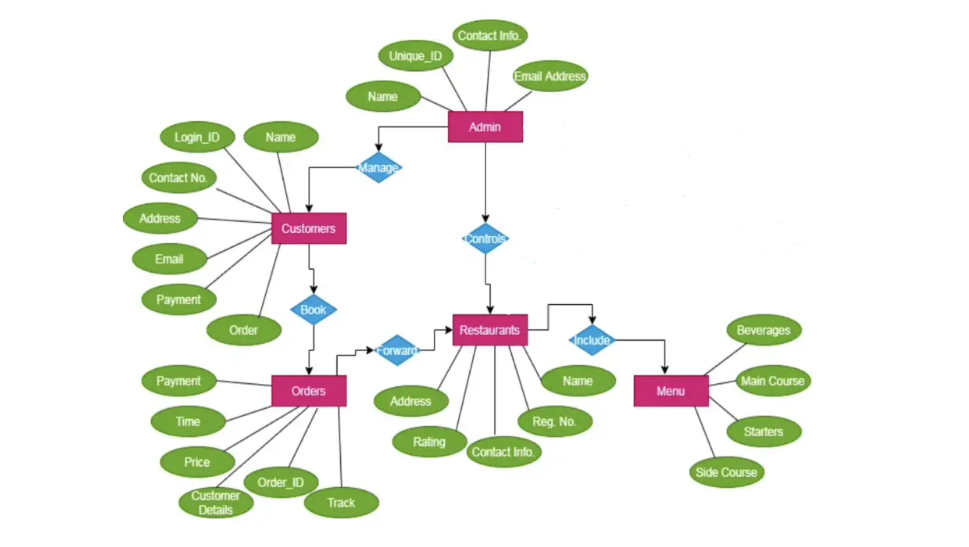
\includegraphics[scale=0.55]{ear.png}
    \caption{Performance Evaluation}
    \label{fig:pereva}
\end{figure}

\subsection{Project Management}
Project management for an online food ordering system:

\textbf{1. Define project scope:}This involves identifying the goals, objectives, and requirements of the online food ordering system. It is essential to understand the target audience, features required, and technology stack required to develop the system.

\textbf{2. Identify project stakeholders:} Project stakeholders include developers, designers, product owners, and project managers. It is essential to ensure that all stakeholders understand the project's scope and expectations to ensure a successful outcome.

\textbf{3. Develop a project plan:} A project plan is crucial to ensure that the project is completed within the defined timeline and budget. The project plan should include a detailed schedule, resource allocation, and risk management plan.

\textbf{4. Develop a prototype:} Developing a prototype will help visualize the system's functionality and ensure that the design meets the user's needs. A prototype can be developed using wireframes or visual designs.

\textbf{5. Implement the system:} This involves developing the system using the chosen technology stack and design. Testing should be done regularly to ensure that the system is functional and meets the project requirements.

\textbf{6. Launch and monitor the system:} Once the system is developed, it needs to be launched and monitored. The monitoring process involves identifying any issues and fixing them in real-time.

\textbf{7. Evaluate the project:} Once the project is completed, it is essential to evaluate the project's success. This evaluation can help identify areas of improvement and inform future project management decisions.

Overall, effective project management of an online food ordering system requires a well-defined scope, stakeholder management, thorough planning, development, monitoring, and evaluation.

\clearpage

